% begin module infinite-limit-ln-tan
\begin{frame}
\begin{columns}
\column{.5\textwidth}
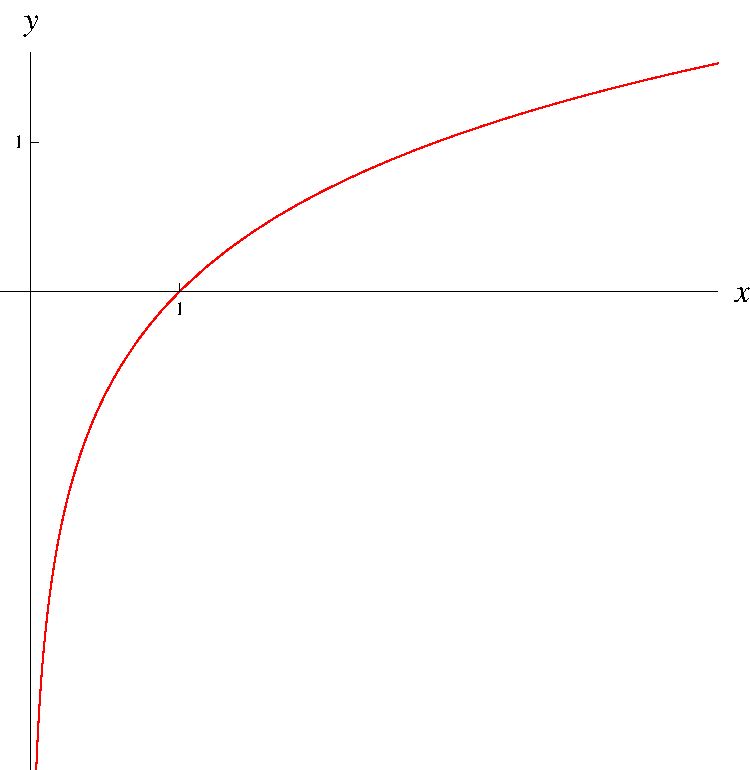
\includegraphics[width=5cm]{limits/pictures/graph-ln.pdf}

\abovedisplayskip=0pt
\belowdisplayskip=-15pt
\abovedisplayshortskip=0pt
\belowdisplayshortskip=0pt
\begin{align*}
\ln x & \invisible{=} \\
\alert<handout:0| 2-3>{\lim_{x\to 0^+}\ln x} & \alert<handout:0| 2-3>{= \uncover<3->{-\infty}} \\
\alert<handout:0| 4-5>{\lim_{x\to 0^-}\ln x} & \alert<handout:0| 4-5>{= \uncover<5->{\text{DNE}}} \\
\alert<handout:0| 6-7>{\lim_{x\to 0}\ln x} & \alert<handout:0| 6-7>{= \uncover<7->{\text{DNE}}} \\
\end{align*}
\column{.5\textwidth}
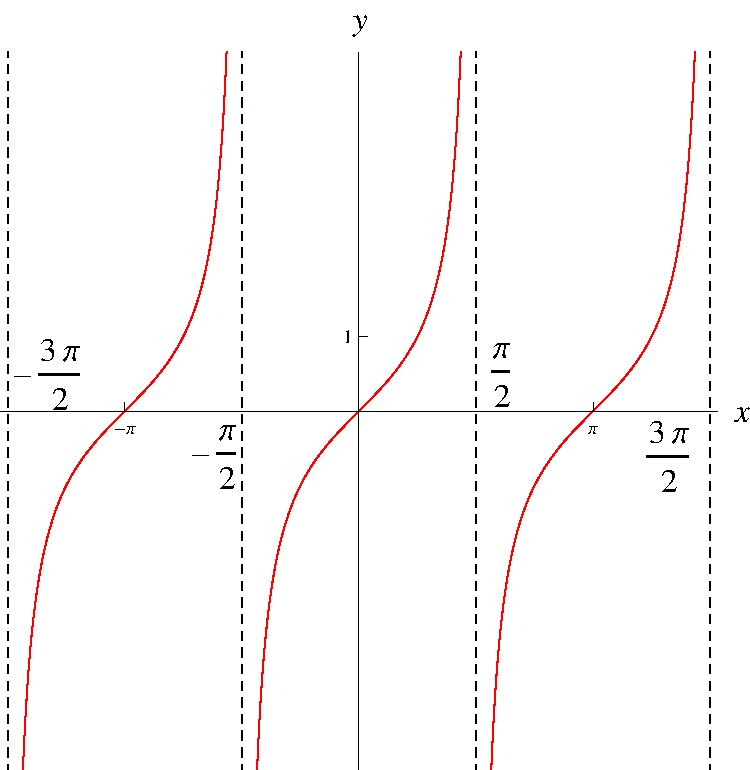
\includegraphics[width=5cm]{limits/pictures/graph-tan.pdf}

\abovedisplayskip=0pt
\belowdisplayskip=-15pt
\abovedisplayshortskip=0pt
\belowdisplayshortskip=0pt
\begin{align*}
\tan x & \invisible{=} \\
\alert<handout:0| 8-9>{\lim_{x\to \pi/2^+}\tan x} & \alert<handout:0| 8-9>{= \uncover<9->{-\infty}} \\
\alert<handout:0| 10-11>{\lim_{x\to \pi/2^-}\tan x} & \alert<handout:0| 10-11>{= \uncover<11->{\infty}} \\
\alert<handout:0| 12-13>{\lim_{x\to \pi/2}\tan x} & \alert<handout:0| 12-13>{= \uncover<13->{\text{DNE}}} \\
\end{align*}
\end{columns}
\end{frame}
% end module infinite-limit-ln-tan
